% ##### INIZIO PREAMBOLO ##### %

% ----- Stile del documento (tipo, margini, etc..) ----- %

% Tipo di documento
\documentclass[a4paper, twoside, titlepage, 11pt]{article}

% Setto i margini (il bindingoffset � lo spazio per la rilegatura)
\usepackage[includehead, headheight=1cm, headsep=0.5cm, top=2cm, bottom=2cm, left=2cm, right=2cm, bindingoffset=0.5cm]{geometry}

% Per gli spazi di interlinea
\usepackage{setspace}
\onehalfspacing

% Per i caption (ad esempio i titoli delle figure)
\usepackage[bf,footnotesize]{caption}

% ----- Fine stile del documento ----- %


% ----- Intestazioni ----- %

% Header di default delle pagine
\usepackage{fancyhdr}
\pagestyle{fancy}
\renewcommand{\sectionmark}[1]{\markright{\thesection\ \ #1}}
\fancyhf{}
\fancyhead[LE,RO]{\bfseries\thepage}
\fancyhead[RE,LO]{\bfseries\rightmark}

% Header per le pagine della TOC
\fancypagestyle{toc}{ \fancyhf{} \pagenumbering{roman} \fancyhead[LO,RE]{\bf{Indice}} \fancyhead[LE,RO]{\bfseries \thepage}}

% Header per le pagine della bibliografia
\fancypagestyle{bibliografia}{ \fancyhf{} \fancyhead[LO,RE]{\bf{Bibliografia e sitografia}} \fancyhead[LE,RO]{\bfseries \thepage}}

% ----- Fine intestazioni ----- %


% ----- Internazionalizzazione ----- %

% Per l'italiano (ad esempio per la sillabazione)
\usepackage[italian]{babel}

% Per poter usare i caratteri speciali italiani (vedi lettere accentate)
\usepackage[latin1]{inputenc}

% ----- Fine internazionalizzazione ----- %


% ----- Immagini o tabelle ----- %

% Per inserire file .eps
\usepackage[dvips]{graphicx}

% Per i flottanti
\usepackage{floatflt}

\usepackage{verbatim}
% ----- Fine immagini o tabelle ----- %


% ----- Per gli indici ----- %

% Per l'indice analitico
\usepackage{makeidx}
\makeindex

% Per avere l'indice analitico cliccabile (deve essere l'ultimo pacchetto caricato)
%\usepackage[colorlinks=true, pdfborder={0 0 0}]{hyperref}

% ----- Fine indici ----- %

% ----- Info sul documento ----- %

\title{Plugin MySQL dissector per nProbe}
\author{Emanuele Tomasi}

% ----- Fine info sul documento ----- %


% ##### FINE PREAMBOLO ##### %



% ##### INIZIO DOCUMENTO ##### %

\begin{document}

% ----- PRIMA PAGINA (il titolo del documento) ----- %
\maketitle

% ----- SECONDA PAGINA (l'indice TOC) ----- %
\newpage
\thispagestyle{toc}
\tableofcontents

% ----- L'ARTICOLO ----- %
\newpage
\pagenumbering{arabic}

\section{Uno sguardo a \emph{nProbe}}
Sviluppato da Luca Deri, \emph{nProbe} � una sonda che implementa il protocollo \emph{NetFlow} (il nome infatti sta per \emph{NetFlow probe}). A partire dalla versione 9 di \emph{NetFlow}, le informazioni esportate non sono pi� standardizzate secondo quanto stabilito da Cisco (creatore del protocollo), ma sono scelte dall'utente attraverso un \emph{template}. Grazie all'uso dei \emph{template}, quindi, le informazioni generate da \emph{nProbe} non sono solo le classiche 7-tuple:

\begin{enumerate}
\item indirizzo IP sorgente
\item indirizzo IP destinatario
\item porta sorgente
\item porta destinazione
\item protocollo IP
\item interfaccia di ingresso (SNMP ifIndex)
\item IP Type of Service (\emph{ToS})
\end{enumerate}
ma ve ne possono essere anche altre aggiuntive e/o sostitutive.

\subsection{La struttura a plugin di \emph{nProbe}}
\emph{nProbe} implementa questi nuovi protocolli con un insieme di plugin esterni al codice principale e tutti inseriti nella directory {\footnotesize \texttt{plugins}}. Ogni plugin � in grado di esportare una o pi� informazioni identificate da un \emph{id} e un \emph{nome} univoci. Al momento dell'invocazione, l'utente sceglie cosa vuole esportare usando l'opzione:

\begin{footnotesize}
\begin{verbatim}
[--flow-templ|-T] <flow template>   | Specify the NFv9 template
\end{verbatim}
\end{footnotesize}
\emph{nProbe}, quindi, va alla ricerca dei plugin che implementano almeno una tra le informazioni richieste nel \emph{template} e li attiva.

Ad esempio, un plugin attualmente presente � l'\emph{SMTP Protocol Dissector} che nell'help di \emph{nProbe} riporta quanto segue:

\begin{footnotesize}
\begin{verbatim}
Plugin SMTP Protocol Dissector templates:
[NFv9 57657][IPFIX 35632.185] %SMTP_MAIL_FROM           Mail sender
[NFv9 57658][IPFIX 35632.186] %SMTP_RCPT_TO             Mail recipient
\end{verbatim}
\end{footnotesize}
In questo esempio, il plugin pu� esportare sia il mittente che il destinatario di una email. L'\emph{id} univoco che attiva il plugin richiedendogli di esportare il mittente � 57657 (per \emph{NetFlow v.9}. Invece � 35632\footnote{35632 � il \emph{Private Enterprise Number (PEN)} assegnato a \emph{ntop} dall'\emph{Internet Assigned Numbers Authority (IANA)}. Anche \emph{ntop} � stato sviluppato da Luca Deri.}.185 per il protocollo \emph{IPFIX}\footnote{L'\emph{Internet Protocol Flow Information Export (IPFIX)} � un protocollo standardizzato dall'\emph{Internet Engineering TaskForce (IETF)} basato su \emph{NetFlow v.9}.}), mentre il \emph{nome} univoco da inserire nel \emph{template} � {\footnotesize \texttt{\%SMTP\_MAIL\_FROM}}. Se si vuole attivare il plugin richiedendogli di esportare il destinatario della email, basta inserire nel \emph{template} la stringa {\footnotesize \texttt{\%SMTP\_RCPT\_TO}}. Il comando seguente, quindi, fa attivare il plugin \emph{SMTP Protocol Dissector} e gli chiede di esportare nel flusso sia il mittente che il destinatario di una email\footnote{In realt� questo \emph{template} � veramente minimale ed � a solo scopo di esempio. Se non si inseriscono nel \emph{templata} le informazioni relativa agli indirizzi, alle porte e al protocollo IP, \emph{nProbe} ignora totalmente queste informazioni e non riesce a riconoscere i flussi in maniera corretta.}:

\begin{footnotesize}
\begin{verbatim}
nprobe -T "%SMTP_MAIL_FROM %SMTP_RCPT_TO"
\end{verbatim}
\end{footnotesize}

\subsection{Cosa scrivere nei plugin}
Dovendo stare ``staccato'' dal codice principale, un plugin deve implementare delle funzioni dai prototipi ben definiti ed essere in grado di fornire gli indirizzi di queste funzioni a \emph{nProbe}, in modo tale che quest'ultimo sia poi in grado di eseguirle ogniqualvolta lo ritenga necessario.

\subsubsection{L'interfaccia dei plugin}
Tutte le informazioni su di un plugin sono inserite nella struttura dati {\footnotesize \texttt{PluginInfo}}, dichiarata come segue nel file {\footnotesize \texttt{engine.h}}:

\begin{footnotesize}
\begin{verbatim}
typedef struct pluginInfo {
  char *nprobe_revision, *name, *version, *descr, *author;
  u_char always_enabled, enabled;
  PluginInitFctn initFctn;
  PluginTermFctn termFctn;
  PluginConf pluginFlowConf;
  PluginFctn deleteFlowFctn;
  u_char call_packetFlowFctn_for_each_packet;
  PluginPacketFctn packetFlowFctn;
  PluginGetPluginTemplateFctn getPluginTemplateFctn;
  PluginCheckPluginExportFctn checkPluginExportFctn;
  PluginCheckPluginPrintFctn checkPluginPrintFctn;
  PluginSetupFctn setupFctn;
  PluginHelpFctn helpFctn;
} PluginInfo;
\end{verbatim}
\end{footnotesize}
Le variabili il cui tipo inizia con ``Plugin'' sono dei puntatori a funzione il cui prototipo � dichiarato sempre nello stesso file. Le prime cinque variabili di tipo stringa sono informazioni sul plugin:

\begin{description}
\item[{\footnotesize nprobe\_revision}] la revisione di \emph{nProbe} per cui � scritto il plugin. Se questo viene aggiornato al pari del programma principale si pu� anche usare la costante {\footnotesize \texttt{NPROBE\_REVISION}}.
\item[{\footnotesize name}] il nome del plugin.
\item[{\footnotesize version}] la versione.
\item[{\footnotesize descr}] la sua descrizione.
\item[{\footnotesize author}] le informazioni sullo sviluppatore.
\end{description}

Dopo queste informazioni seguono due variabili booleane:

\begin{description}
\item[{\footnotesize always\_enabled}] indica se il plugin deve essere attivo indipendentemente dal \emph{template} utente (settata a 1) oppure deve essere attivato esclusivamente se richiesto nel \emph{template} (settata a 0).
\item[{\footnotesize enabled}] � una variabile per uso interno. Indica se il plugin � stato attivato o meno.
\end{description}

Infine gli altri elementi della struttura che, come gi� detto, sono principalmente dei puntatori a funzione. Se si decide di non implementare una o pi� di queste funzioni, basta settare il loro valore a {\footnotesize \texttt{NULL}}:

\begin{description}
\item[{\footnotesize initFctn}] viene invocata per inizializzare il plugin. \emph{nProbe} passa a questa funzione l'intera command line, in modo tale che un plugin possa andare alla ricerca di qualche parametro che gli interessa (si veda la funzione {\footnotesize \texttt{helpFctn()}}).
\item[{\footnotesize termFctn}] opposta alla precedente {\footnotesize \texttt{initFctn()}}, viene invocata per terminare il plugin.
\item[{\footnotesize pluginFlowConf}] tutte le informazioni che un plugin pu� esportare, come detto, sono caratterizzate da un \emph{id} e da un \emph{nome} ma oltre a questi due attributi ne esistono altri che \emph{nProbe} usa internamente. Questa funzione, ritorna un'array terminato da un entry particolare, con tutti gli attributi associati ad ogni informazione che il plugin � in grado di esportare. Si capir� meglio quando si vedr� come fa il plugin ad informare \emph{nProbe} su quali informazioni � in grado di esportare.
\item[{\footnotesize deleteFlowFctn}] viene invocata quando si elimina un flusso. Ad esempio, in questa funzione il plugin pu� liberare eventuale memoria allocata associata al flusso.
\item[{\footnotesize call\_packetFlowFctn\_for\_each\_packet}] questa variabile, di tipo booleano, indica se si vuole chiamare la funzione {\footnotesize \texttt{packetFlowFctn()}} per ogni pacchetto del flusso (settata ad 1), oppure solo per il primo pacchetto del flusso (settata a 0).
\item[{\footnotesize packetFlowFctn}] � la funzione principale che viene invocata al ricevimento di ogni pacchetto appartenente al flusso (si veda la variabile precedente {\footnotesize \texttt{call\_packetFlowFctn\_for\_each\_packet}}). � in questa funzione che il plugin estrae le informazioni.
\item[{\footnotesize getPluginTemplateFctn}] questa funzione prende il nome di un elemento del \emph{template} utente (un elemento della stringa passata con l'opzione {\footnotesize \texttt{-T}}) e, se il plugin lo gestisce, ritorna tutti gli attributi ad esso associati, altrimenti ritorna {\footnotesize \texttt{NULL}}. Anche questa funzione sar� pi� chiara una volta che si vedr� come fa il plugin ad informare \emph{nProbe} su quali informazioni � in grado di esportare.
\item[{\footnotesize checkPluginExportFctn}] viene invocata al momento dell'esportazione dei dati. In questa funzione il plugin scrive in un buffer limitato, quelle informazioni richieste nel \emph{template} che � in grado di gestire.
\item[{\footnotesize checkPluginPrintFctn}] \emph{nProbe} su richiesta pu� salvare le informazioni esportate anche in un file temporaneo e, quando lo fa, invoca questa funzione. � simile alla precedente funzione {\footnotesize \texttt{check\-Plugin\-Export\-Fctn()}}, solo che in questo caso siccome i dati sono scritti in un file, non c'� limite alle informazioni che si possono scrivere. Ad esempio, se il mittente di una email � troppo lungo, potrebbe essere necessario troncare questa informazione per farla entrare nel buffer da esportare, mentre non vi sono restrizioni quando l'informazione � scritta nel file temporaneo.
\item[{\footnotesize setupFctn}] viene invocata subito dopo l'inizializzazione di tutti i plugin, poco prima che \emph{nProbe} inizi la cattura dei pacchetti.
\item[{\footnotesize helpFctn}] viene invocata durante l'esecuzione dell'help di \emph{nProbe} (parametro {\footnotesize \texttt{--help|-h}}) per mostrare le opzioni necessarie al plugin. Se un utente, invocando \emph{nProbe}, gli passa sulla command line una o pi� tra queste opzioni, il plugin le pu� intercettare durante l'esecuzione della funzione {\footnotesize \texttt{initFctn()}}.
\end{description}

\subsubsection{Far avere l'interfaccia ad \emph{nProbe}}
Una volta che nel codice del plugin viene definita la struttura {\footnotesize \texttt{PluginInfo}}, si deve farla avere ad \emph{nProbe}. Per fare questo ci sono due modi, a seconda che i plugin vengano inseriti staticamente nel binario compilato, oppure vengano caricati dinamicamente a tempo di esecuzione. In ogni caso, si deve implementare una funzione senza parametri che ritorna un puntatore alla struttura {\footnotesize \texttt{PluginInfo}} definita, questa sar� la cerniera tra il plugin e il codice principale. Nel primo caso, in cui i plugin sono inseriti nel binario a tempo di compilazione, si deve inserire nel file {\footnotesize \texttt{plugin.c}} la dichiarazione della funzione esterna (definita nel plugin) che restituir� la struttura dati. Ad esempio, per il plugin di SMTP nel file c'� inserita questa dichiarazione:

\begin{footnotesize}
\begin{verbatim}
#ifdef MAKE_STATIC_PLUGINS
...
extern PluginInfo* smtpPluginEntryFctn(void)
...
#endif
\end{verbatim}
\end{footnotesize}

Invece, nel caso in cui i plugin sono caricati in maniera dinamica a tempo di esecuzione, \emph{nProbe} deve sapere a priori il nome della funziona da invocare una volta caricato il codice, cos� il plugin deve definire, al suo interno, la funzione:

\begin{footnotesize}
\begin{verbatim}
PluginInfo *PluginEntryFctn(void)
\end{verbatim}
\end{footnotesize}
La figura \ref{load-plugin-a-runtime} mostra come vengono prelevate le interfacce dei plugin, quando questi vengono inseriti a tempo di esecuzione.
\begin{figure}[ht]
    \centering
    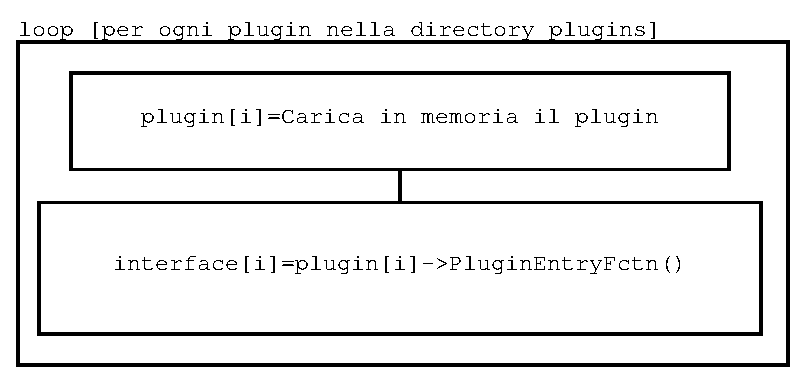
\includegraphics[scale=0.8]{images/caricamento_plugin_dinamici.eps}
    \caption{Prelevamento interfacce plugin a run-time}
    \label{load-plugin-a-runtime}
\end{figure}

\subsubsection{Le informazioni esportate}
Una volta che il plugin � correttamente legato al codice di \emph{nProbe} non resta che una cosa da fare, indicare a quest'ultimo quando attivarlo. Come gi� detto, \emph{nProbe} si basa sul \emph{template} utente passato attraverso il parametro {\footnotesize \texttt{-T}} della linea di comando per sapere quale plugin attivare e quale no. Per ogni informazione che il plugin � in grado di esportare, si deve definire una struttura {\footnotesize \texttt{V9V10TemplateElementId}}, dichiarata nel file {\footnotesize \texttt{nprobe.h}} come segue:

\begin{footnotesize}
\begin{verbatim}
typedef struct flow_ver9_ipfix_template_elementids {
  u_int8_t  isOptionTemplate; /* 0=flow template, 1=option template */
  u_int8_t  useLongSnaplen;
  u_int32_t templateElementEnterpriseId;
  u_int16_t templateElementId;
  u_int8_t variableFieldLength;
  u_int16_t templateElementLen;
  ElementFormat elementFormat; /* Only for elements longer than 4 bytes */
  ElementDumpFormat fileDumpFormat; /* Hint when data has to be printed on
                                       a human readable form */
  char      *templateElementName, *templateElementDescr;
} V9V10TemplateElementId;
\end{verbatim}
\end{footnotesize}
Le variabili della struttura hanno il seguente significato:

\begin{description}
\item[{\footnotesize isOptionTemplate}] Specifica se il \emph{template} � un \emph{option template} (settata a 1) o un \emph{flow template} (settata a 0). Si possono usare le due costanti {\footnotesize \texttt{FLOW\_TEMPLATE}} e {\footnotesize \texttt{OPTION\_TEMPLATE}}, definite in {\footnotesize \texttt{nprobe.h}} come segue:

\begin{footnotesize}
\begin{verbatim}
#define FLOW_TEMPLATE       0
#define OPTION_TEMPLATE     1
\end{verbatim}
\end{footnotesize}
\item[{\footnotesize useLongSnaplen}] \emph{nProbe} � in grado di passare al plugin tutto il \emph{payload} del pacchetto oppure solo una piccola parte. Nel caso in cui un plugin voglia fare \emph{packet inspection} e necessiti di tutto il \emph{payload} contenuto nel pacchetto deve settare questa opzione a 1, altrimenti se necessita solo di una piccola parte iniziale pu� settare questa opzione a 0. Alternativamente ai valori numerici si possono usare le costanti definite nel file {\footnotesize \texttt{nprobe.h}}:

\begin{footnotesize}
\begin{verbatim}
#define SHORT_SNAPLEN       0
#define LONG_SNAPLEN        1
\end{verbatim}
\end{footnotesize}
Si noti che anche nel caso in cui questa opzione � settata a {\footnotesize \texttt{LONG\_SNAPLEN}}, il \emph{payload} ha comunque una dimensione massima che non pu� andare oltre il valore della costante:

\begin{footnotesize}
\begin{verbatim}
#define PCAP_LONG_SNAPLEN        1600
\end{verbatim}
\end{footnotesize}
definita nel file {\footnotesize \texttt{engine.h}}.
\item[{\footnotesize templateElementEnterpriseId}] l'identificativo univoco dell'azienda che ha creato il plugin (ad esempio il \emph{PEN} rilasciato dalla \emph{IANA}).
\item[{\footnotesize templateElementId}] l'identificativo univoco per questa informazione (il suo \emph{id}).
\item[{\footnotesize variableFieldLength}] specifica se l'informazione ha dimensione fissa o variabile. Anche in questo caso si pu� usare una delle due costanti {\footnotesize \texttt{STATIC\_FIELD\_LEN}} o {\footnotesize \texttt{VARIABLE\_FIELD\_LEN}}, definite in {\footnotesize \texttt{nprobe.h}} come segue:

\begin{footnotesize}
\begin{verbatim}
#define STATIC_FIELD_LEN    1
#define VARIABLE_FIELD_LEN  2
\end{verbatim}
\end{footnotesize}

\item[{\footnotesize templateElementLen}] la dimensione massima, in byte, che occupa quest'informazione. Anche se la precedente variabile {\footnotesize \texttt{variableFieldLength}} � stata settata a {\footnotesize \texttt{VARIABLE\_FIELD\_LEN}}, occorre comunque informare {\footnotesize \texttt{nProbe}} della sua dimensione massima.
\item[{\footnotesize elementFormat}] specifica il formato di questa informazione. Il tipo di questa variabile � {\footnotesize \texttt{Element\-Format}}, che � un \emph{enumerate} definito sempre in {\footnotesize \texttt{nprobe.h}}:

\begin{footnotesize}
\begin{verbatim}
typedef enum {
  ascii_format = 0,
  hex_format,
  numeric_format,
  ipv6_address_format
} ElementFormat;
\end{verbatim}
\end{footnotesize}
\item[{\footnotesize fileDumpFormat}] indica come dev'essere stampata l'informazione in un formato interpretabile dall'uomo. Il tipo di questa variabile � {\footnotesize \texttt{ElementDumpFormat}}, che  � un \emph{enumerate} definito in {\footnotesize \texttt{nprobe.h}} come segue:

\begin{footnotesize}
\begin{verbatim}
typedef enum {
  dump_as_uint = 0, /* 1234567890 */
  dump_as_formatted_uint, /* 123'456 */
  dump_as_ip_port,
  dump_as_ip_proto,
  dump_as_ipv4_address,
  dump_as_ipv6_address,
  dump_as_mac_address,
  dump_as_epoch,
  dump_as_bool,
  dump_as_tcp_flags,
  dump_as_hex,
  dump_as_ascii
} ElementDumpFormat;
\end{verbatim}
\end{footnotesize}
\item[{\footnotesize templateElementName}] il nome univoco che identifica questa informazione (quello che viene usato nel \emph{template} utente passato con l'opzione {\footnotesize \texttt{-T}}).
\item[{\footnotesize templateElementDescr}] una descrizione sull'informazione che si esporta.
\end{description}

� molto importante scegliere bene sia la variabile {\footnotesize \texttt{templateElementId}} che {\footnotesize \texttt{template\-Element\-Name}} perch�, come detto, devono essere univoche. Per la seconda si usa anteporre il nome del plugin in modo da stare relativamente sicuri (ad esempio: {\footnotesize \texttt{SMTP\_MAIL\_FROM}} o {\footnotesize \texttt{SMTP\_RCPT\_TO}}). Per la prima invece bisogna assicurarsi che l'\emph{id} non sia gi� stato usato. L'unica informazione usabile � una base di partenza, definita nel file {\footnotesize \texttt{nprobe.h}} dalla costante {\footnotesize \texttt{NTOP\_BASE\_ID}}:

\begin{footnotesize}
\begin{verbatim}
#define NTOP_BASE_ID 57472
\end{verbatim}
\end{footnotesize}

Dato che un plugin generalmente esporta pi� di un'informazione, queste strutture {\footnotesize \texttt{V9V10\-Template\-Element\-Id}} devono essere inserite in un'array terminato dalla particolare struttura:

\begin{footnotesize}
\begin{verbatim}
{ FLOW_TEMPLATE, NTOP_ENTERPRISE_ID, 0, STATIC_FIELD_LEN, 0, 0, 0, NULL, NULL }
\end{verbatim}
\end{footnotesize}

Ora si possono capire meglio le due funzioni dell'interfaccia dei plugin, {\footnotesize \texttt{pluginFlowConf()}} e {\footnotesize \texttt{get\-Plugin\-Template\-Fctn()}}. La prima ritorna l'array contenente tutte le strutture dati {\footnotesize \texttt{V9V10\-Template\-Element\-Id}} per le informazioni definite dal plugin, mentre la seconda prende come parametro il nome di un'informazione, controlla per ogni struttura la variabile {\footnotesize \texttt{templateElementName}}, e se ne trova una uguale al parametro passatogli, allora ritorna il puntatore alla struttura {\footnotesize \texttt{V9V10\-Template\-Element\-Id}} associata, altrimenti ritorna {\footnotesize \texttt{NULL}}.

\emph{nProbe}, per sapere se deve attivare un plugin o meno, esegue l'algoritmo seguente (si veda la figura \ref{attivazione_plugin}): per ogni elemento passato nel \emph{template} utente tramite l'opzione {\footnotesize \texttt{-T}}, invoca la funzione {\footnotesize \texttt{getPluginTemplateFctn()}} di un plugin e, se questo ritorna una struttura {\footnotesize \texttt{V9V10TemplateElementId}} valida (cio� diversa da {\footnotesize \texttt{NULL}}), lo attiva.

\begin{figure}[ht]
    \centering
    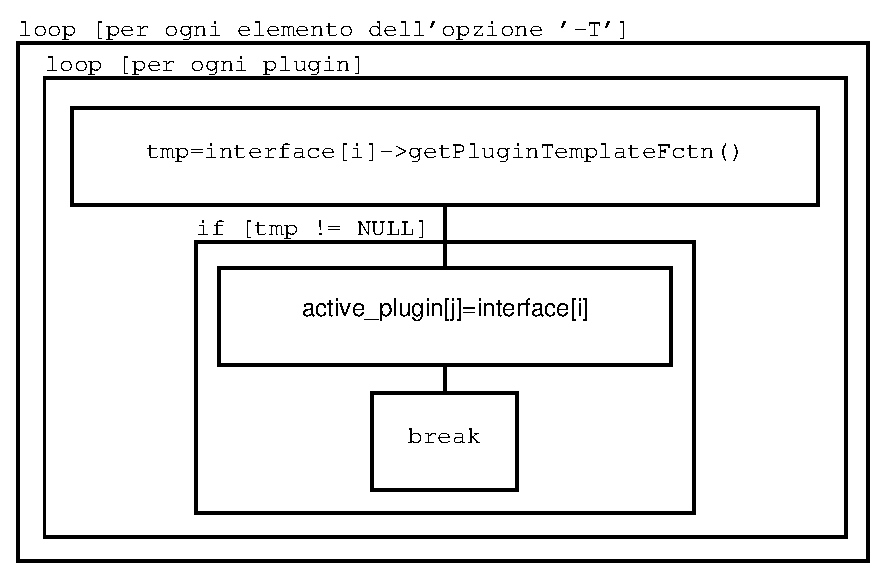
\includegraphics[scale=0.8]{images/attivazione_plugin.eps}
    \caption{Algoritmo di attivazione dei plugin}
    \label{attivazione_plugin}
\end{figure}

\subsubsection{I dati privati}
\label{dati_privati}
Alla creazione di un nuovo flusso, \emph{nProbe} crea una struttura dati di tipo {\footnotesize \texttt{FlowHashBucket}} dichiarata nel file {\footnotesize \texttt{bucket.h}}. Questa stuttura dati � molto complessa ed � quasi esclusivamente di uso interno. Per quanto riguarda i plugin tutto ci� che importa sapere � la presenza all'interno di questa struttura dati della variabile {\footnotesize \texttt{plugin}}: una lista concatenata di strutture dati di tipo {\footnotesize \texttt{PluginInformation}}. Se un plugin � interessato ad analizzare il flusso appena creato, deve definire un oggetto di tipo {\footnotesize \texttt{PluginInformation}} e concatenarlo alla lista puntata dalla variabile {\footnotesize \texttt{plugin}}.

Prima di vedere pi� in dettaglio cosa avviene dal punto di vista dei plugin durante la creazione di un nuovo flusso, � importante vedere la struttura dati {\footnotesize \texttt{PluginInformation}} dichiarata sempre nel file {\footnotesize \texttt{bucket.h}}:

\begin{footnotesize}
\begin{verbatim}
typedef struct pluginInformation {
  struct pluginInfo *pluginPtr;
  void *pluginData;
  struct pluginInformation *next;
} PluginInformation;
\end{verbatim}
\end{footnotesize}
La struttura ha tre variabili:

\begin{description}
\item[{\footnotesize pluginPtr}:] un puntatore all'interfaccia del plugin (la sua struttura dati {\footnotesize \texttt{PluginInfo}}).
\item[{\footnotesize pluginData}:] un puntatore a dei dati privati che il plugin vuole associare al flusso.
\item[{\footnotesize next}:] il prossimo elemento della lista.
\end{description}

Durante la creazione di un flusso avviene quanto segue:

\begin{itemize}
\item \emph{nProbe} crea la struttura dati {\footnotesize \texttt{FlowHashBucket}} settando la variabile {\footnotesize \texttt{plugin}} a {\footnotesize \texttt{NULL}}.
\item Per ogni plugin attivo, invoca la funzione {\footnotesize \texttt{packetFlowFctn()}} passandogli la struttura\\ {\footnotesize \texttt{FlowHashBucket}} e una variabile ({\footnotesize \texttt{new\_bucket}}) settata appositamente (a 1) per far capire al plugin che si tratta di un nuovo flusso.
\item Il plugin, se � interessato a trattare il flusso:
  \begin{itemize}
    \item definisce una variabile di tipo {\footnotesize \texttt{PluginInformation}}.
    \item collega alla variabile {\footnotesize \texttt{pluginPtr}} la sua struttura dati {\footnotesize \texttt{PluginInfo}}.
    \item eventualmente crea una struttura dati privata da collegare alla variabile {\footnotesize \texttt{pluginData}}.
    \item si inserisce nella lista concatenata {\footnotesize \texttt{plugin}} di {\footnotesize \texttt{FlowHashBucket}}.
  \end{itemize}
\end{itemize}
In questo modo \emph{nProbe} ha nella variabile {\footnotesize \texttt{plugin}} di ogni flusso, la lista concatenata dei plugin attivi per quello specifico flusso.

Per rendere pi� chiaro ci� che avviene, ecco un estratto dal \emph{MySQL protocol dissector}:

\begin{scriptsize}
\begin{verbatim}
/* La struttura per i dati privati del plugin */
struct plugin_data
{
  ...
};

static void
mysqlPlugin_packet(u_char new_bucket,
		   FlowHashBucket* bkt,
                   u_short sport,
                   u_short dport,
                   ...)
{
  struct plugin_data *p_data; /* dati privati del plugin */

  /* Testa se il flusso � interessante:
     ovvero se almeno una delle porte � quella del server MySQL */
  if ( sport != MYSQL_SERVER_PORT && dport != MYSQL_SERVER_PORT )
    return; /* Nothing to be done */

  ...

  if ( new_bucket ) /* Se � un nuovo flusso */
    {
      /* Crea la struttura dati PluginInformation */
      PluginInformation *info;
      if( ! (info = (PluginInformation*)malloc(sizeof(PluginInformation))) )
        {
          traceEvent(TRACE_ERROR, "Not enough memory?");
          return; /* Not enough memory */
        }

      /* Colloga la sua PluginInfo alla variabile pluginPtr */
      info->pluginPtr  = (void*)&mysqlPlugin;

      /* Crea la struttura per i dati privati e la collega alla variabile pluginData */
      if ( ! (p_data = info->pluginData = malloc(sizeof(struct plugin_data))) )
        {
          traceEvent(TRACE_ERROR, "Not enough memory?");
          free(info);
          return; /* Not enough memory */
        }

      /* Collega le sue informazioni alla lista dei plugin attivi per questo flusso */
      info->next = bkt->plugin;
      bkt->plugin = info;
    }
\end{verbatim}
\end{scriptsize}

\subsubsection{Esportazione forzata delle informazioni}
L'esportazione delle informazioni su di un flusso � generalmente segnata dalla ``morte'' del flusso stesso o quando lo si ritiene scaduto. Questo per� permette di ottenere solo delle informazioni aggregate sul flusso e non delle informazioni specifiche: si pu� sapere quanti byte in totale si sono scambiati server e client e non cosa si sono scambiati in un dato momento.

\emph{nProbe} mette a disposizione dei plugin una funzione che forza l'esportazione delle informazioni pur eventualmente mantenendo in memoria i dati interni relativi al flusso stesso. La funzione � definita nel file {\footnotesize \texttt{engine.c}} ed ha il seguente prototipo:

\begin{footnotesize}
\begin{verbatim}
void exportBucket(FlowHashBucket *myBucket, u_char free_memory);
\end{verbatim}
\end{footnotesize}

Dove {\footnotesize \texttt{myBucket}} � il flusso che si vuole esportare, mentre {\footnotesize \texttt{free\_memory}} � una variabile booleana che, se settata a 1 indica di rimuovere dalla memoria le informazioni sul flusso\footnote{Attenzione a settare la variabile a 1. Questo implica la chiamata per ogni plugin attivo su quel flusso della funzione \texttt{deleteFlowFctn()} e la rimozione da parte di \emph{nProbe} della struttura dati \texttt{FlowHashBucket}. Se per� il flusso non � effettivamente terminato, l'arrivo di nuovi dati implicheranno la creazione di un nuovo flusso con tutto l'iter che ne consegue.}, mentre se viene settata a 0 i dati relativi al flusso rimarranno comunque in memoria.

L'esportazione di un flusso implica l'invocazione per ogni plugin attivo su quel flusso della sua funzione {\footnotesize \texttt{checkPluginExportFctn()}}, ed eventualmente della funzione {\footnotesize \texttt{checkPluginPrintFctn()}}. In questo modo il plugin � in grado di dire al collezionatore cosa si sono scambiati in un determinato periodo il server e il client.

\subsubsection{Un plugin di base}
Per riassumere tutto ci� che si � visto in questo paragrafo, ecco il corpo vuoto di un plugin:

\raggedbottom
\begin{scriptsize}
\verbatiminput{includes/plugin_base.c}
\end{scriptsize}
\flushbottom

\subsection{Cosa tenere a mente durante la stesura di un plugin}
Va ricordato che \emph{nProbe} � una sonda e cattura i pacchetti che passano dalla rete. Durante lo sviluppo di un plugin per l'analisi di un particolare protocollo, si deve tener sempre presente che il plugin:

\begin{itemize}
\item \texttt{Deve essere stateless}. La sonda in generale non riceve i pacchetti cos� come li ricevono gli host che generano il flusso. Il client e il server sanno in ogni istante cosa aspettarsi dal pacchetto successivo, ma la sonda potrebbe essere stata attivata, ad esempio, nel mezzo della comunicazione. Pertanto � un errore scrivere un plugin che implementa un automa a stati per l'analisi del contenuto. Affermazioni come: ``dato che prima � passato il pacchetto A, questo � sicuramente il pacchetto B'', sono, in generale, sbagliate.
\item \texttt{Deve stare attento alla frammentazione dei pacchetti}. Un flusso di informazioni potrebbe non essere inviato tutto in un solo pacchetto. Se, ad esempio, il client e il server usano una connessione TCP e il client invia una richiesta superiore al \emph{maximum transmission unit (MTU)}, allora il kernel del client suddivider� il flusso di richiesta in pi� pacchetti TCP. Il kernel del server dall'altra parte ``fonder�'' questi pacchetti e li far� ricevere all'applicazione come un unico flusso di dati continuo. Questa suddivisione del flusso �, quindi, completamente trasparente alle applicazioni client e server, ma il plugin, per quanto detto al punto precedente, deve occuparsi anche di questa eventualit�. Non solo la sonda potrebbe aver perso uno dei pacchetti, ma tenendo conto dell'inaffidabilit� della rete, potrebbe prendere i pacchetti in un ordine casuale, oppure prendere un duplicato del pacchetto precedente\footnote{Ad esempio se il protocollo di trasporto � TCP e un pacchetto non viene ricevuto.}.
\item \texttt{Non si deve fidare dei pacchetti}. Il plugin non deve basarsi solo sulle specifiche del protocollo per analizzare i pacchetti, ma deve stare sempre attento che ci� che analizza sia effettivamente un pacchetto valido. Ad esempio, se nelle specifiche del protocollo viene detto che una stringa e null-terminated, il plugin potrebbe usare una strlen() per contare quanto � grande la stringa, ma se non tiene conto del fatto che il pacchetto che sta analizzando potrebbe non essere di quel protocollo e che, quindi, il carattere di fine stringa potrebbe non esserci affatto, allora la strlen() potrebbe andare in buffer overflow determinando un segmentation fault del plugin e il conseguente crash della sonda.
\end{itemize}

% LocalWords:  nProbe Deri NetFlow Cisco template tuple SNMP ifIndex Type of TO
% LocalWords:  Service ToS plugin plugins SMTP Protocol Dissector Enterprise
% LocalWords:  Number PEN ntop dall' Assigned Numbers Authority IANA IPFIX Flow
% LocalWords:  Information TaskForce IETF PluginInfo engine nprobe revision for
% LocalWords:  name version descr author always enabled NULL initFctn command
% LocalWords:  line helpFctn termFctn pluginFlowConf un'array entry call each
% LocalWords:  deleteFlowFctn packetFlowFctn packet getPluginTemplateFctn Fctn
% LocalWords:  checkPluginExportFctn checkPluginPrintFctn setupFctn run option
% LocalWords:  TemplateElementId isOptionTemplate flow useLongSnaplen payload
% LocalWords:  inspection LONG SNAPLEN templateElementEnterpriseId STATIC FIELD
% LocalWords:  templateElementId variableFieldLength LEN VARIABLE elementFormat
% LocalWords:  templateElementLen Element Format fileDumpFormat FROM RCPT get
% LocalWords:  ElementDumpFormat templateElementName templateElementDescr next
% LocalWords:  l'array FlowHashBucket bucket stuttura PluginInformation new TCP
% LocalWords:  pluginPtr pluginData MySQL dissector morte' client myBucket host
% LocalWords:  memory collezionatore includes router stateless transmission MTU
% LocalWords:  unit fonder�' null terminated strlen overflow segmentation fault
% LocalWords:  crash

\section{Il protocollo MySQL}
In questo paragrafo verr� analizzato, a grandi linee, il protocollo MySQL\footnote{Maggiori informazioni possono essere prelevate dal sito:\\http://forge.mysql.com/wiki/MySQL\_Internals\_ClientServer\_Protocol}. Questo permetter� di capire in che modo funziona il plugin per l'analisi dei pacchetti MySQL e da dove preleva le informazioni che esporta (l'username dell'utente che si collega al server, il database che sta interrogando, etc\ldots).

� importante notare fin da subito che esistono delle differenze sostanziali tra le versioni minori e quelle maggiori o uguali alla 4.1 del protocollo. Alcune di queste differenze sono trasparenti allo scopo del plugin, altre, come si vedr�, saranno gestite.

\subsection{L'handshake}
Dopo l'handshake a livello TCP, viene effettuato un secondo handshake a livello di protocollo MySQL. In questa fase vengono inviati esattamente i 3 pacchetti\footnote{In questo contesto i pacchetti sono intesi come pacchetti del protocollo MySQL.} seguenti:

\begin{enumerate}
\item Il server, tra le altre cose, informa il client sulla propria versione, sulla versione del protocollo che � in grado di gestire, sul linguaggio accettato e sull'identificativo del thread che gestisce la connessione. Questo pacchetto � conosciuto come \emph{greeting packet}.
\item Il client a sua volta invia al server delle informazioni utili per la connessione, come ad esempio la dimensione massima dei pacchetti, in byte, che � in grado di accettare. Oltre a queste informazioni, invia anche le credenziali dell'utente (username e password) necessarie per l'autenticazione\footnote{L'autenticazione in realt� inizia dal \emph{greeting packet} ed � differente a seconda che vengano usati protocolli inferiori al 4.1 oppure no.}. Per quest'ultimo motivo il pacchetto viene conosciuto come \emph{client authentication packet} o \emph{login packet}. Se entrambi, client e server, gestiscono la versione 4.1 del protocollo\footnote{Si noti che in questa fase, il client sa gi� quale versione del protocollo sar� usata, perch� conosce sia la sua, che quella del server (che gli � stata inviata nel \emph{greeting packet}).}, allora in questo pacchetto il client pu� inviare anche il nome del database sul quale intende lavorare. Ancora, il formato del pacchetto � differente a seconda che si usino delle versioni superiori o uguali alla 4.1 del protocollo, oppure no.
\item Il server conclude l'handshake inviando al client un pacchetto chiamato \emph{result packet}. Se � in grado di soddisfare le richieste del client e l'autenticazione � avvenuta con successo, la connessione va avanti, altrimenti il server nega l'accesso e chiude la connessione.
\end{enumerate}
Sia il server (nel \emph{greeting packet}) che il client (nel \emph{login packet}) inviano una maschera di bit di 2 byte che contiene svariate informazioni, tra cui un flag che indica se sono in grado di gestire il protocollo 4.1 o superiore. La maschera inviata dal server viene chiamata \emph{server\_capabilities}, mentre quella inviata dal client prende il nome di \emph{client\_flag} e, nel caso in cui il protocollo usato � il 4.1 o superiore, dopo \emph{client\_flag} il client invia altri 2 byte conosciuti come \emph{client\_extended\_flag}.

\subsection{L'header dei pacchetti}
Tutti i pacchetti MySQL hanno un'intestazione fissa di 4 byte. I primi 3 byte indicano la dimensione, in byte, del pacchetto stesso e, dato che questa informazione � un numero intero non negativo, la dimensione massima di un pacchetto MySQL � di $2^{24}=16$MB. Ai fini del plugin, questo vuol dire che un pacchetto MySQL pu� essere frammentato in pi� pacchetti TCP.

L'ultimo byte dell'intestazione indica il numero di sequenza del pacchetto. Questo numero viene azzerato alla fine di ogni comunicazione. Quindi, ad esempio, i tre pacchetti dell'handshake sono numerati 0, 1 e 2 e, dopo di ci�, la sequenza viene riazzerata.

\subsection{I pacchetti di richiesta (\emph{command packet})}
Se l'handshake � avvenuto con successo, il client pu� iniziare a interrogare il server inviando dei pacchetti conosciuti come \emph{command packet}. Il primo byte di questo pacchetto identifica il comando, mentre i rimanenti byte ne sono l'argomento.

\subsection{I pacchetti di risposta (\emph{result packet})}
\label{result_packet}
Ricevuta la richiesta dal client, il server risponde con quello che viene chiamato genericamente un \emph{result packet} (come quello che termina l'handshake). Il primo byte di questo pacchetto � chiamato \emph{field\_count} e identifica il tipo di risposta che il server da al client. A seconda del valore del \emph{field\_count} questo pacchetto viene chiamato:

\begin{description}
\item[\footnotesize{Ok Packet:}]{indica che tutto � andato bene, lo si riconosce perch� il \emph{field\_count} � 0x00.}
\item[\footnotesize{Error Packet:}]{indica che c'� stato un errore, lo si riconosce perch� il \emph{field\_count} � 0xFF.}
\item[\footnotesize{Result Set Header Packet:}]{� l'intestazione del risultato di una query. Il \emph{field\_count} ha un valore compreso tra 0x01 a 0xFD e indica il numero di colonne della tabella risultante\footnote{Potrebbe sembrare che il numero di colonne del risultato sia al pi� 253 (0xFD). In realt� questo singolo byte pu� anche indicare quanti byte successivi devono essere presi per calcolare un numero intero che arriva sino a $2^{64}$.}.}
\end{description}
Nel caso di un \texttt{Result Set Header Packet}, il server invier� tutti i pacchetti (incrementando sempre il numero di sequenza) che permetteranno al client di ottenere l'intera tabella del risultato della query. Il server invier� dapprima tanti pacchetti per quanto era il valore del \emph{field\_count} del \texttt{Result Set Header Packet}. Questa prima serie di pacchetti, ognuno dei quali � chiamato \emph{Field Packet}, definisce i campi delle colonne della tabella (ad esempio, id di tipo intero, nome di tipo stringa, etc\ldots). La fine di questa prima serie di pacchetti viene decretata dall'invio del pacchetto chiamato \emph{EOF Packet} (il cui primo byte vale 0xFE) che, a volte, pu� servire per trasportare delle informazioni. Il server quindi invia al client un'altra serie di pacchetti chiamati \emph{Data Packet}, ognuno dei quali contiene una riga della tabella (quindi il valore della prima colonna, il valore della seconda colonna, etc\ldots). Ed infine, per terminare la sequenza dei \emph{Data Packet} il server invia un altro pacchetto di \emph{EOF Packet}.

La figura \ref{mysql-protocol} mostra un esempio di connessione MySQL in cui, dopo l'handshake, il client seleziona un database ed esegue una SELECT. Si noti come, grazie alle informazioni ricevute, il client � in grado di creare la tabella risultante.

\begin{figure}[htbp]
    \centering
    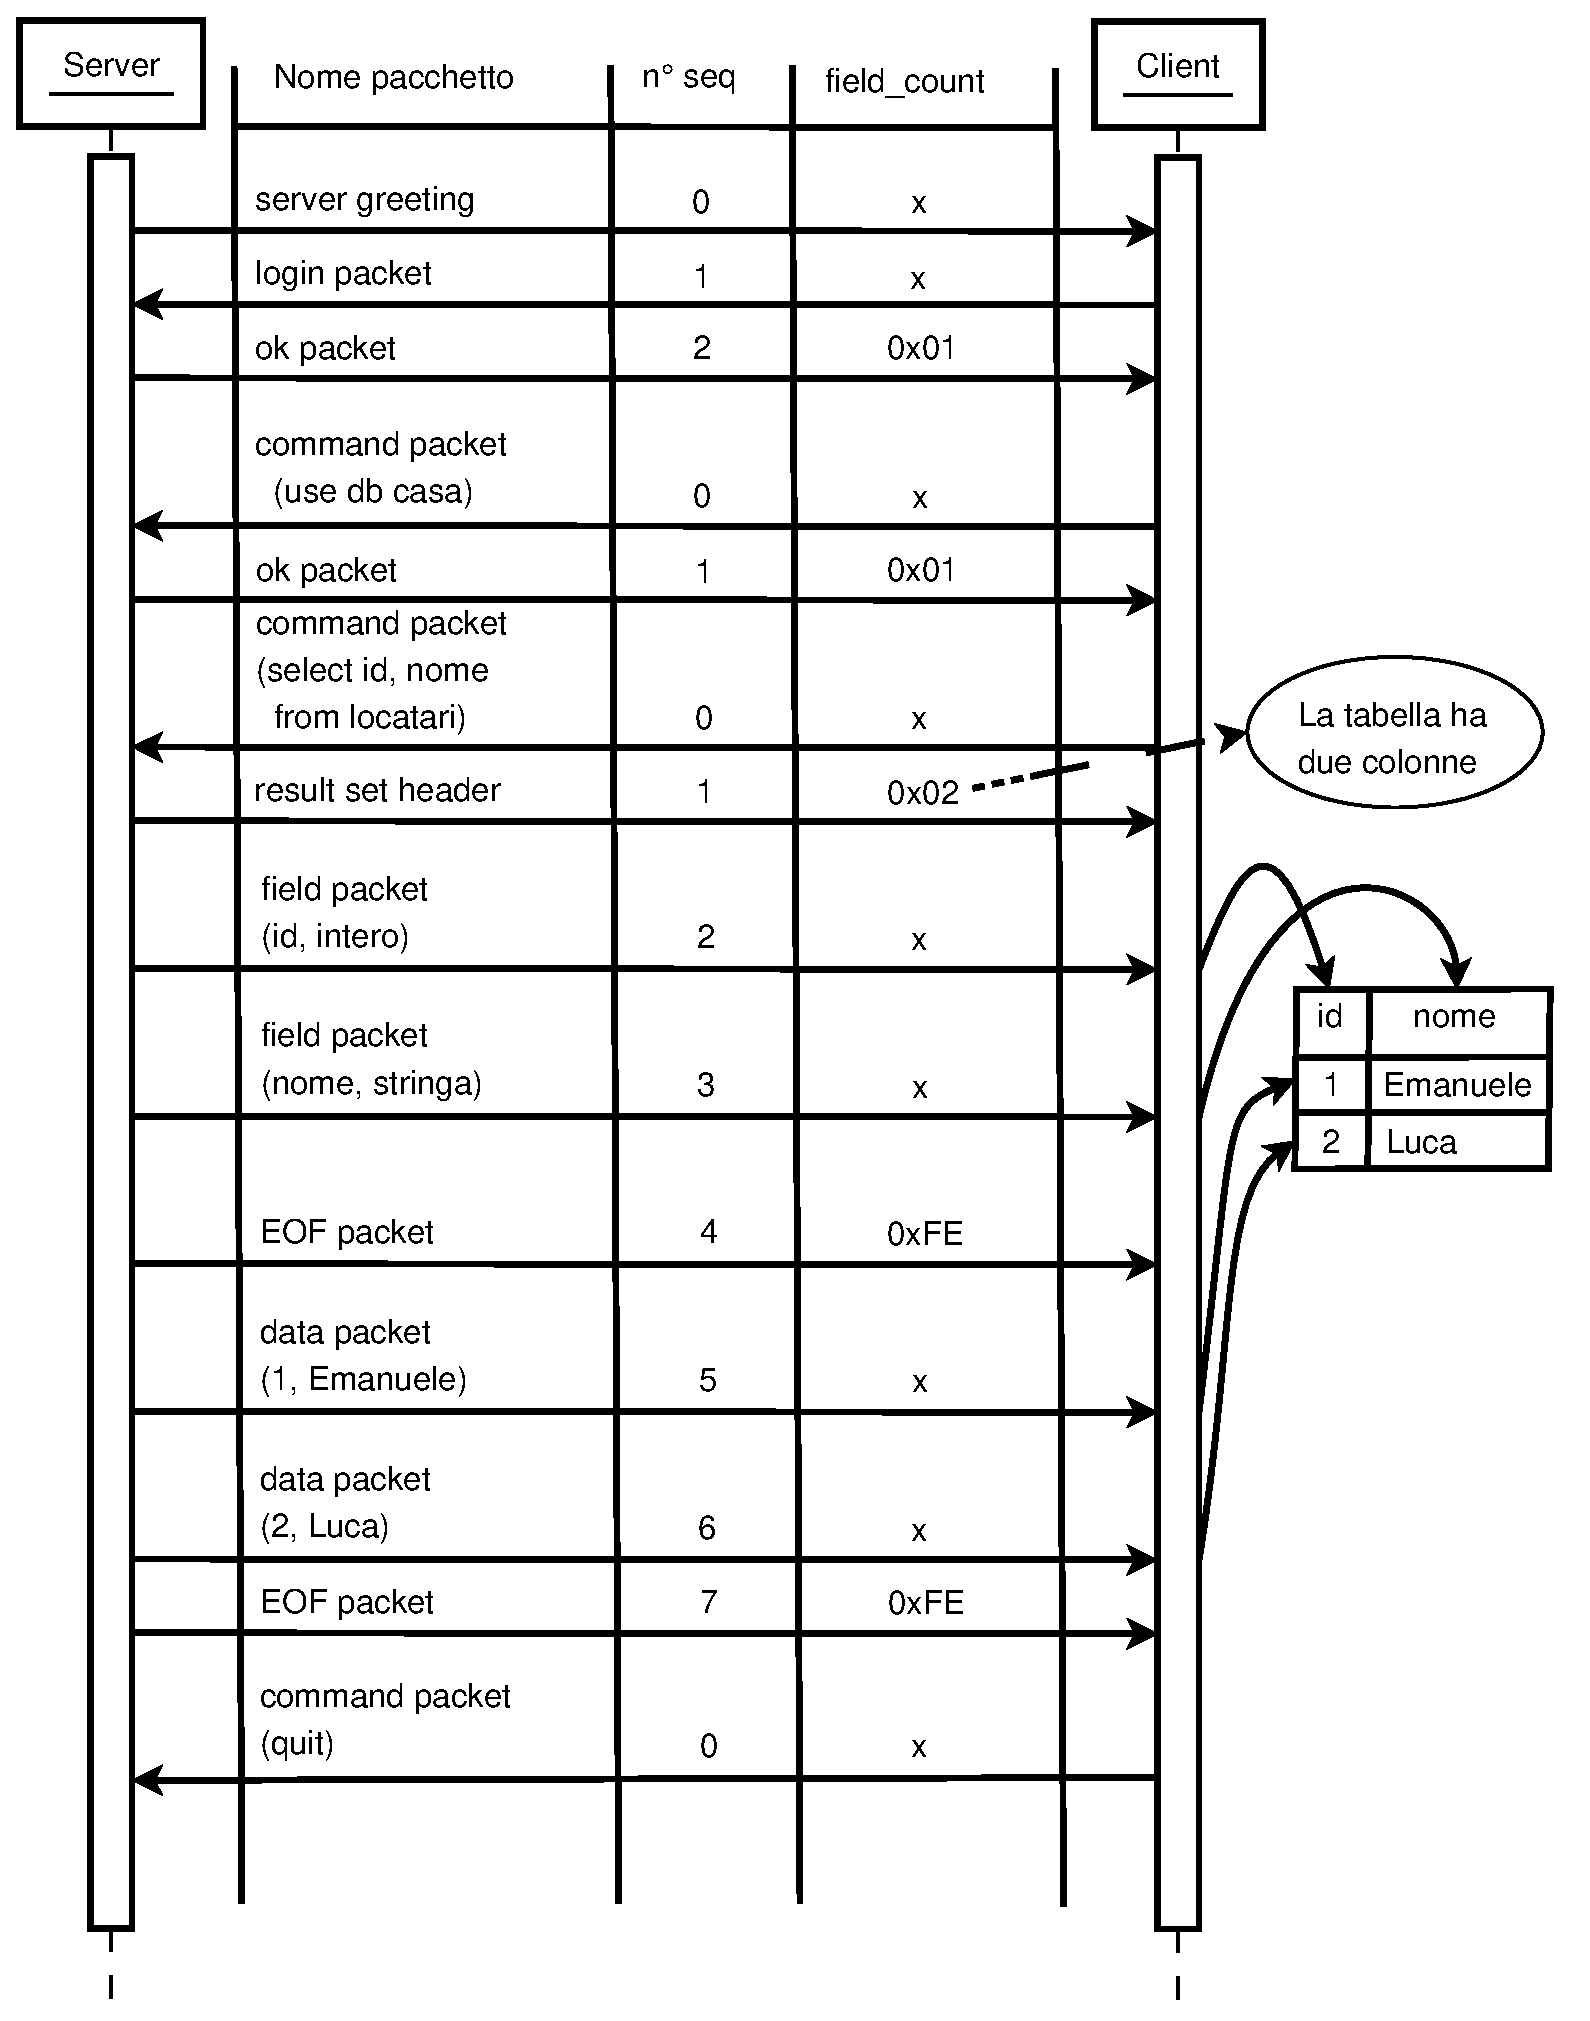
\includegraphics[scale=0.62]{images/mysql_protocol.eps}
    \caption{Esempio di una connessione MySQL}
    \label{mysql-protocol}
\end{figure}

% LocalWords:  MySQL Internals ClientServer Protocol plugin l'username TCP MB
% LocalWords:  L'handshake l'handshake handshake client thread greeting packet
% LocalWords:  username authentication result capabilities L'header riazzerata
% LocalWords:  dell'handshake command field count Error xFF Header query xFD
% LocalWords:  EOF xFE SELECT

\section{Il plugin \emph{MySQL Protocol Dissector}}
Dopo il background acquisito su \emph{nProbe} e sul protocollo MySQL si pu� passare a vedere il plugin \emph{MySQL protocol dissector}.

\subsection{Le informazioni esportate}
Attualmente il plugin � in grado di esportare le seguenti informazioni sul traffico MySQL (sono i nomi univoci da passare a \emph{nProbe} come parte del \emph{template}):

\begin{description}
\item[{\footnotesize MYSQL\_SERVER\_VERSION:}] la versione del server MySQL. Viene passata dal server al client nel \emph{greeting packet}.
\item[{\footnotesize MYSQL\_USERNAME:}] il nome dell'utente che si � collegato al server. Viene passato dal client al server nel \emph{login packet}.
\item[{\footnotesize MYSQL\_DB:}] il database al quale si � attualmente collegati. Ci sono due modi in cui il client seleziona un database: se server e client gestiscono il protocollo di versione superiore o uguale al 4.1, il client pu� selezionare un database direttamente nel \emph{login packet}; altrimenti il client invia un \emph{command packet} il cui comando � \emph{use database}.
\item[{\footnotesize MYSQL\_REQUEST:}] la versione human-readable della richiesta fatta dal client. Come detto, il primo byte del \emph{command packet} identifica il comando che il client chiede di eseguire al server. Qui viene esportata una versione pi� leggibile di questa richiesta cos�, ad esempio, se il primo byte vale 0x03, e cio� se il client sta chiedendo al server di eseguire una query al database, l'informazione esportata sar� la stringa: ``Query''.
\item[{\footnotesize MYSQL\_QUERY:}] l'eventuale query che deve essere eseguita. Sono tutti i byte successivi al primo del \emph{command packet} nel caso in cui il primo byte valga 0x03.
\item[{\footnotesize MYSQL\_REQUEST:}] la risposta del server. E' il \emph{field\_count} (il primo byte) del \emph{result packet} che, come si � visto, ha significati differenti a seconda della richiesta fatta dal client.
\end{description}

Queste informazioni vengono esportate dal plugin ad ogni \emph{result packet}. Se l'handshake viene catturato tutto correttamente si pu� quindi sapere la versione del server MySQL, l'username dell'utente, l'eventuale database selezionato nel \emph{login packet} e la risposta del server che informa il client se la connessione � stata accettata o meno. Durante l'esecuzione normale di richiesta-risposta tra client e server invece, si possono analizzare la richiesta fatta dal client con l'eventuale query e il suo esisto.

\subsection{L'analisi del traffico}
Dalle specifiche del protocollo MySQL e dalle informazioni che il plugin � in grado di esportare, si nota che tutto ci� che serve si trova all'inizio del pacchetto. Per risolvere il problema della frammentazione del pacchetto MySQL in pi� pacchetti TCP e di tutto quello che ne consegue (ritrasmissione dei pacchetti TCP errati, riordino dei pacchetti TCP, etc\ldots), il plugin tiene in memoria solo il primo (o meglio parte del primo) degli eventuali pacchetti TCP diretti dal client al server, o viceversa.

Il plugin riconosce la fine di una serie di pacchetti TCP quando la direzione cambia; questo perch� il server non risponde sino a che tutti i pacchetti TCP non gli sono stati recapitati con successo (ovvero fino a che non ha ricostruito tutto il pacchetto MySQL), e viceversa, il client non richiede l'esecuzione di un altro comando se non ha letto tutte le risposte del server. Sino a che la direzione del ``discorso'' non cambia, il plugin si preoccupa solo di controllare che il pacchetto TCP che la sonda cattura non sia precedente a quello che lui pensa essere il primo della serie; questo avviene quando la rete mischia i pacchetti TCP facendoli arrivare in disordine alla sonda. Quando poi la direzione cambia, il plugin effettua l'analisi del pacchetto in memoria ed eventualmente esegue l'esportazione delle informazioni. Vale la pena notare che il pacchetto precedente non � sempre quello con il numero di sequenza minore, infatti, il numero di sequenza � un numero positivo intero ma a 32 bit, il fatto che sia limitato superiormente implica che prima o poi questo numero ricomincer� dall'inizio e, se questo avviene, il primo pacchetto non � pi� quello che ha il numero di sequenza pi� piccolo in assoluto, ma quello con il numero di sequenza pi� piccolo tra quelli pi� grandi. Per tenere conto di questa eventualit�, il controllo effettuato dal plugin � il seguente:

\begin{footnotesize}
\begin{verbatim}
if ( tcpSeqNum < p_data->tcp_info.firstPktSeqNum &&
	     (tcpSeqNum + 8388608) > p_data->tcp_info.firstPktSeqNum )
  /* E' un nuovo primo */
\end{verbatim}
\end{footnotesize}
Si controlla che il numero di sequenza attuale ({\footnotesize \texttt{tcpSeqNum}}) sia effettivamente pi� piccolo di quello che il plugin pensa essere il primo pacchetto della serie ({\footnotesize \texttt{p\_data->tcp\_info.firstPktSeqNum}}). Inoltre si controlla che aggiungendo al numero di sequenza del pacchetto attuale, un numero relativamente grande ($2^{23} = 8388608$), questo risulti effettivamente pi� grande di quello salvato, cosa che non avviene nel caso in cui il numero di sequenza � stato resettato\footnote{Si ricordi che il numero di sequenza va di pari passo con i byte inviati. Un pacchetto MySQL come detto in precedenza non pu� essere pi� grande di $2^{24}$ byte quindi, nell'eventualit� che il numero di sequenza sia stato resettato, aggiungendo $2^{23}$ a questo numero non lo far� mai essere pi� grande del pi� piccolo tra i pi� grandi.}.

Ovviamente osservare il flusso del ``discorso'' implica che il plugin non � completamente stateless in quanto si aspetta di vedere un cambio di direzione. L'analisi del traffico TCP per� � molto complicata e potrebbe portare via molte risorse. Si ricordi che il plugin gira su una sonda che potrebbe avere attivi innumerevoli flussi nello stesso periodo di tempo, i plugin non devono quindi ``rubare'' molte risorse per compiere il loro lavoro. L'algoritmo scelto � sembrato essere un buon compromesso tra efficienza e coerenza dei dati esportati, infatti, se ad esempio la sonda dovesse perdere l'unico pacchetto TCP che segna il cambio del ``discorso'', quello che succede � che il plugin pensa che la direzione non sia mai cambiata e quindi le informazioni che esporta in un dato momento potrebbero essere errate. Questo per� non ha impatto sul futuro, dove se non ci sono altri errori di cattura, il plugin si riallineer� al ``discorso''.

\subsubsection{In ritardo di uno}
L'analisi del pacchetto viene effettuata, come detto, solo al cambio di direzione del ``discorso'' tra il client e il server. Nel momento in cui il flusso scade per�, questo cambio di direzione non avviene, ed il plugin deve tener conto anche di questa eventualit�. \emph{nProbe} invoca comunque le funzioni {\footnotesize \texttt{exportFcnt()}} e {\footnotesize \texttt{printFcnt()}} quando il flusso � scaduto e durante l'esecuzione di queste funzioni, quindi, va controllato se il pacchetto conservato in memoria � stato analizzato oppure no, altrimenti si rischia di esportare delle informazioni vecchie.

\subsection{Le strutture dati private}
Durante l'analisi del traffico MySQL si possono individuare tre tipi di dati distinti:

\begin{description}
\item[I dati statici della connessione MySQL:] quei dati che vengono scambiati durante l'handshake e che rimangono uguali per tutta la connessione\footnote{Tra queste informazioni il plugin mette anche l'username dell'utente collegato al database. In realt� esiste un comando chiamato \emph{change user} che permette di cambiare l'utente a connessione avviata.}.
\item[I dati relativi alla connessione TCP:] sono i dati necessari a seguire il ``discorso'' a livello di pacchetti TCP.
\item[I dati dinamici della connessione MySQL:] quali ad esempio, il comando richiesto dal client, l'eventuale query, la risposta al comando, etc\ldots.
\end{description}
Per ognuno di questi tipi di dati il plugin ha una struttura dati ben definita:

\begin{scriptsize}
\begin{verbatim}
/* Informazioni statiche della connessione MySQL (prelevate durante l'handshake) */
struct mysql_connection_info
{
  char *mysql_server_version;   /* la versione del server */
  char *mysql_username;         /* l'username dell'utente collegato */
  u_int16_t s_caps;             /* server capability */
  u_int16_t c_caps;             /* client capability (client flag) */
  u_int16_t c_ext_caps;         /* ciente extended capability (client extended flag) */
};

/* Informazioni del flusso TCP */
struct mysql_tcp_info
{
  u_short src_port;                                  /* porta sorgente */
  u_int32_t firstPktSeqNum;                          /* numero di sequenza del primo pacchetto */
  u_char firstPktPayload[MYSQL_TCP_PKT_MAX_SIZE+1];  /* primo pacchetto del "discorso" (primi byte) */
  int firstPktPayloadLen;                            /* dimensione, in byte, del primo pacchetto salvato */
  u_char wasDissected;                               /* il pacchetto � stato analizzato (1) o no (0)? */
};

/* Struttura dati privata collegata al flusso
 * (contiene le informazioni dinamiche della connessione MySQL).
 */
struct plugin_data
{
  char *mysql_db;                       /* il database attualmente in uso */
  u_int8_t mysql_command;               /* comando di cui client chiede l'esecuzione */
  char *mysql_query;                    /* eventuale query fatta dal client */
  int16_t mysql_response;               /* risposta del server (si notino i 2 byte) */
  struct mysql_connection_info c_info;  /* informazioni statiche sul flusso MySQL */
  struct mysql_tcp_info tcp_info;       /* informazioni sul flusso TCP */
};
\end{verbatim}
\end{scriptsize}
Il plugin collega solo la struttura {\footnotesize \texttt{plugin\_data}} alla variabile {\footnotesize \texttt{pluginData}} della {\footnotesize \texttt{PluginInformation}} relativa al flusso (si veda \ref{dati_privati}), le altre strutture dati come si vede sono contenute in essa sotto forma di variabili.

C'� un altra struttura dati che il plugin usa durante l'analisi del pacchetto MySQL, quella che contiene le informazioni sull'header:

\begin{scriptsize}
\begin{verbatim}
/* Header del pacchetto MySQL */
struct mysql_packet_header
{
  u_int32_t length; /* dimensione del pacchetto (solo 24 bit) */
  u_char number;    /* numero di sequenza del pacchetto */
};
\end{verbatim}
\end{scriptsize}

\subsection{Il plugin in azione}
Ecco l'output prodotto dall'esecuzione di \emph{nProbe} su un pacchetto MySQL grazie all'ausilio del plugin:

\begin{scriptsize}
\begin{verbatim}
$> nprobe -p 1/1/1/1/0/1 -T "%PROTOCOL %IPV4_SRC_ADDR %IPV4_DST_ADDR %L4_SRC_PORT %L4_DST_PORT\
   %MYSQL_SERVER_VERSION %MYSQL_USERNAME %MYSQL_DB %MYSQL_REQUEST %MYSQL_QUERY %MYSQL_RESPONSE"\
   -P /tmp -i ../samples/mysql_complete.pcap
05/Oct/2010 11:00:28 [nprobe.c:2548] Welcome to nprobe v.5.8.2 ($Revision: 1700 $) for\
                                     x86_64-unknown-linux-gnu
05/Oct/2010 11:00:28 [nprobe.c:2600] Dumping flow files every 60 sec into directory /tmp
05/Oct/2010 11:00:28 [nprobe.c:2606] WARNING: -n parameter is missing. 127.0.0.1:2055 will be used.
05/Oct/2010 11:00:28 [plugin.c:137] Loading plugins [.so] from ./plugins
05/Oct/2010 11:00:28 [dbPlugin.c:72] Initializing DB plugin
05/Oct/2010 11:00:28 [util.c:295] GeoIP: loaded AS config file GeoIPASNum.dat
05/Oct/2010 11:00:28 [plugin.c:580] 1 plugin(s) enabled
05/Oct/2010 11:00:28 [plugin.c:511] Enabling plugin MySQL Protocol Dissector
05/Oct/2010 11:00:28 [engine.c:1695] Saving flows into temporary file '/tmp/2010/10/05/11/00.flows.temp'
05/Oct/2010 11:00:29 [engine.c:1554] Flow file '/tmp/2010/10/05/11/00.flows' is now available

$> sed -n '1 b print;/|56162|3306|/b print;d;:print {s/\([^|]*|\)\{5\}//;p;}' /tmp/2010/10/05/11/00.flows
MYSQL_SERVER_VERSION|MYSQL_USERNAME|MYSQL_DB|MYSQL_REQUEST|MYSQL_QUERY|MYSQL_RESPONSE
5.0.54|tfoerste||Query|select @@version_comment limit 1|1
5.0.54|tfoerste||Query|SELECT DATABASE()|1
5.0.54|tfoerste|test|Use Database||0
5.0.54|tfoerste|test|Query|show databases|1
5.0.54|tfoerste|test|Query|show tables|1
5.0.54|tfoerste|test|Show Fields||3
5.0.54|tfoerste|test|Query|create table foo (id BIGINT( 10 ) UNSIGNED NOT NULL AUTO_INCREMENT PRIMARY KEY,\
                           animal VARCHAR(64) NOT NULL, name VARCHAR(64) NULL DEFAULT NULL) ENGINE = MYISAM|0
5.0.54|tfoerste|test|Query|insert into foo (animal, name) values ("dog", "Goofy")|0
5.0.54|tfoerste|test|Query|insert into foo (animal, name) values ("cat", "Garfield")|0
5.0.54|tfoerste|test|Query|select * from foo|3
5.0.54|tfoerste|test|Query|delete from foo where name like '%oo%'|0
5.0.54|tfoerste|test|Query|delete from foo where id = 1|0
5.0.54|tfoerste|test|Query|select count(*) from foo|1
5.0.54|tfoerste|test|Query|select * from foo|3
5.0.54|tfoerste|test|Query|delete from foo|0
5.0.54|tfoerste|test|Query|drop table foo|0
5.0.54|tfoerste|test|Quit||-1
\end{verbatim}
\end{scriptsize}

Alcuni piccoli commenti sull'output:

\begin{itemize}
\item Per le prime due righe\footnote{Queste due query sono eseguite automaticamente dal client MySQL senza che l'utente abbia ancora iniziato a fare richieste.} di output manca il nome del database in uso, questo vuol dire che durante l'handshake il client non ha selezionato nessun database.
\item La terza riga indica che l'utente ha chiesto di utilizzare il database \emph{test} e il server ha risposto con un \emph{Ok packet} (\emph{field\_count} = 0x00).
\item Una query interessante � riportata dal seguente output:

\begin{scriptsize}
\begin{verbatim}
5.0.54|tfoerste|test|Query|select * from foo|3
\end{verbatim}
\end{scriptsize}
dal quale si riesce a capire che la tabella \emph{foo} contiene tre colonne (coerentemente con la \emph{CREATE TABLE} precedente), pur non essendo state direttamente selezionate dal client durante la \emph{SELECT}.
\item L'ultima riga di output, riporta una risposta come '-1' mentre tutte le risposte del server vanno, come visto nel paragrafo \ref{result_packet}, da 0 (\emph{Ok packet}) a 255 (\emph{Error packet}). Il plugin riserva due byte per le risposte del server in modo da contenere non solo tutti i valori da 0 a 255 ma anche altri con significato speciale. Ogni volta che esporta delle informazioni, il plugin resetta alcuni dati delle strutture private ed uno di questi � proprio la variabile che contiene la risposta del server che viene settata ad un valore sconosciuto di '-1'; questo valore quindi indica che il server non ha risposto, ed in effetti, se si guarda la figura \ref{mysql-protocol}, si nota che alla richiesta di fine sessione da parte del client, il server non risponde ma chiude direttamente la connessione.
\end{itemize}

% LocalWords:  plugin MySQL Protocol Dissector nProbe protocol dissector client
% LocalWords:  template VERSION greeting packet USERNAME DB command REQUEST TCP
% LocalWords:  human readable query Query' field count result l'handshake l'username
% LocalWords:  tcpSeqNum tcp info firstPktSeqNum stateless exportFcnt printFcnt
% LocalWords:  change pluginData PluginInformation sull'header foo table SELECT
% LocalWords:  Error


% ----- Fine ----- %
\end{document}

% ##### FINE DOCUMENTO ##### %